\documentclass[sigconf, nonacm=true, natbib=false]{acmart}
\usepackage[utf8]{inputenc}
\usepackage{amsmath}
\usepackage{amssymb}
\usepackage[style=ACM-Reference-Format,backend=bibtex,sorting=none]{biblatex}
\usepackage{bytefield}
\usepackage{msc}
\usepackage{tikz}
\setmsckeyword{}

\addbibresource{references.bib}

\begin{document}

% Metadata & header
\title{Networking Architecture for Real-time Multiplayer Games}
\author{Sami Kukkonen}
\affiliation{%
  \institution{University of Helsinki}
}

\maketitle

\section{Introduction}
In this assignment, the task is to design a networking architecture for a multiplayer game that is played in real time.
The architecture will need to be able to scale up in case the number of participants grows, reflect the actions of other
users quickly and allow the user to download new game data of arbitrary sizes (\emph{patches}). It is assumed that direct peer-to-peer
connections is not always possible as players might have firewall or NAT enabled, which would block ingressing. The
solution presented here does not make other assumptions about the game mechanics and is specifically focused on the
networking protocol.

\section{Network topology}

\begin{figure}
  \centering
  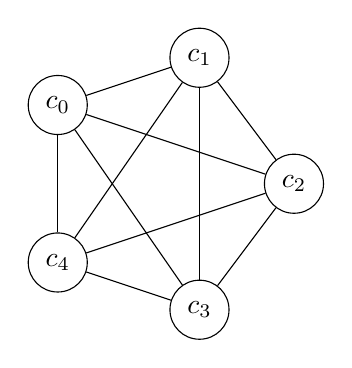
\begin{tikzpicture}
    [scale=.8,auto=left, every node/.style={circle,draw, minimum size=0.75cm}]
    \node (c0) at (0.75, 3.25) {$c_0$};
    \node (c1) at (3, 4) {$c_1$};
    \node (c2) at (4.5, 2) {$c_2$};
    \node (c3) at (3, 0) {$c_3$};
    \node (c4) at (0.75, 0.75) {$c_4$};
    
    \draw (c0) -- (c1);
    \draw (c0) -- (c2);
    \draw (c0) -- (c3);
    \draw (c0) -- (c4);
    \draw (c1) -- (c2);
    \draw (c1) -- (c3);
    \draw (c1) -- (c4);
    \draw (c2) -- (c3);
    \draw (c3) -- (c4);
    \draw (c2) -- (c4);
  \end{tikzpicture}
  
  \caption{Peer-to-peer network topology}
  \label{fig:topo-p2p}
\end{figure}

\begin{figure}
  \centering
  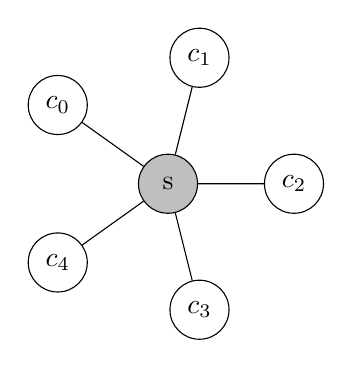
\begin{tikzpicture}
    [scale=.8,auto=left, every node/.style={circle,draw, minimum size=0.75cm}]
    \node (c0) at (0.75, 3.25) {$c_0$};
    \node (c1) at (3, 4) {$c_1$};
    \node (c2) at (4.5, 2) {$c_2$};
    \node (c3) at (3, 0) {$c_3$};
    \node (c4) at (0.75, 0.75) {$c_4$};
    \node[fill=lightgray] (s) at (2.5, 2) {s};
    \draw (c0) -- (s);
    \draw (c1) -- (s);
    \draw (c2) -- (s);
    \draw (c3) -- (s);
    \draw (c4) -- (s);
  \end{tikzpicture}
  \caption{Client-server network topology}
  \label{fig:topo-client-server}
\end{figure}

The network architecture of online multiplayer games can usually be classified into two main topologies: client-server or peer-to-peer.
In client-server architectures, all players (\emph{client nodes}) connect to a \emph{server node} that processes events sent by clients
and broadcasts updated game state to players. In peer-to-peer architecture, nodes communicate directly with each other.
However, peer-to-peer architectures pose scalability issues as the clients in the game session need to be interconnected:
when clients are not in the same LAN, a mechanism for discovering other nodes would be needed. In addition, as each node
has to exchange traffic between all other nodes, the amount of traffic grows quadratically \cite{Smed1} as opposed to linearly
in the client-server architecture. Figures~\ref{fig:topo-p2p}~and~\ref{fig:topo-client-server} provide visualizations for these
two topologies.

Using a central server instead of a peer-to-peer architecture introduces a single point of failure to the system; as the
server is responsible for receiving and broadcasting updates, the capacity of the system is the same as the capacity of
the server. This can be migitated with either vertical or horizontal scaling, e.g. by load balancing packets to multiple
servers and synchronizing state between them.

From a scalability perspective, a peer-to-peer architecture is clearly inferior compared to a client-server model.
In addition, one of the requirements is the ability for the client to download new game configurations; a server is needed
to seed the new data. Given these constraints, we choose to use a client-server topology.


\section{Transport mechanism}
To be able to support game sessions over the Internet, the Internet Protocol suite is chosen as the bottom level of our
networking stack. This gives us two transport protocols to choose from: TCP and UDP. While TCP is best suited for transmissions
where the integrity of data is important, acknowledgement and retransmission of packets might cause significant lag for the client.
This is undesirable for communicating user actions or state updates because they are temporal in nature: an action such as movement or shooting
is dependent on the time in which it is performed. On the other hand, some kind of error recovery is needed for transmitting
new game configurations to clients.

In order to support both temporal and perpetual data streams, we use separate UDP and TCP streams to transmit information.
Temporal state updates will be transmitted via UDP and patches and initial bootstrapping will be transmitted via TCP.

\subsection{Considerations on IP multicasting}

For UDP traffic, it would be possible to use multicasting (routing the same packet to multiple destinations) instead of
unicasting to reduce network traffic on the server. However, this requires substantial infrastructural support and seems
infeasible in practice when communication happens over the Internet \cite{Diot1}. Therefore the server will use
unicasting to communicate with each client.

\section{Error detection and recovery}

UDP adds checksums to sent datagrams, which is used to ensure that the packet integrity is not compromised. However,
the use of checksums is optional for IPv4 packets and required only for IPv6. \cite{rfc2460, rfc8085} To ensure that IPv4 connections
can be used with the game, we add an additional layer of integrity verification by calculating a CRC32 checksum for each
payload and prepending it to the datagram.

Congestion control is another thing that we must consider when using UDP as the transport protocol. Specifically, it is
not guaranteed that UDP packets are delivered at all and if they are, the order of the received packets might not be the
same than when sending. As mentioned before, packet loss is acceptable for temporal data, so we do not implement any
forward error correction mechanisms. If a datagram is detected to be corrupt by a checksum mismatch, it can simply be discarded.
However, out-of-order packets can cause issues when a player's state is replaced by an older state arriving later to the server.

Resiliency against out-of-order deliveries can be achieved with sequence numbering. We use two separate monotonically increasing
integer sequences $i_n$ and $j_n$ for numbering client-originating and server-originating packets, respectively. Now the receiving side
can keep count of the largest received sequence number so far and discard packets with smaller sequence numbers as stale.

To combine integrity protection and loss resiliency, we simply prepend checksums and sequence numbers to the beginning of the datagram.
Thus a basic unit of transmission in the game is a triple $(i, c, d)$ where $i$ is the sequence number, $c$ is the checksum and $d$ is the transmitted data.

\sloppy Let us consider an example that ties up the recovery mechanisms we've introduced: suppose that the client sends three packets
$\langle (1, c_1, d_1), (2, c_2, d_2), (3, c_3, d_3) \rangle$ to the server, but the network link is very unreliable and the server receives
packets $\langle (2, c_2, d_2), (1, c_1, d_1), (3, c_3 + 1, d_3) \rangle$. The first packet is valid, so it is processed and the sequence counter is set to $2$.
The second packet has a sequence number of $1$ and as $1 < 2$ it is considered stale and discarded. The third packet has an invalid checksum, so the
data is assumed to be corrupted and discarded. Now the server has processed $d_2$, which is a correct, although slightly outdated state.

\begin{figure}
  \centering
  \begin{msc}{}

\setlength{\topheaddist}{1cm}
\declinst{c1}{Client}{$c_1$}
\declinst{s}{Server}{$s$}
\declinst{c2}{Client}{$c_2$}

\mess{\textsf{JoinGame}}{c1}{s}
\nextlevel[0.5]
\mess{\textsf{JoinGame}}{c2}{s}
\nextlevel[1]
\mess{game state}{s}{c1}
\nextlevel[0.5]
\mess{game state}{s}{c2}
\nextlevel

\mess*{heartbeat}{c1}{s}
\nextlevel
\mess*{heartbeat}{c2}{s}
\nextlevel

\inlinestart{loop1}{loop}{c1}{c2}
\nextlevel
\settimeout{16ms}{s}[5]
\nextlevel
\regionstart{coregion}{s}
\nextlevel
\mess*{$a_1$}{c1}{s}
\nextlevel
\mess*{$a_2$}{c2}{s}
\nextlevel
\regionend{s}
\nextlevel
\nextlevel
\action*{\textbf{\textsf{UpdateState}}}{s}
\nextlevel[2.5]
\mess*{broadcast}{s}{c1}
\nextlevel[0.5]
\mess*{broadcast}{s}{c2}
\nextlevel
\inlineend{loop1}

\end{msc}
  \caption{Sample message flow between two clients and server}
  \label{fig:msgflow}
\end{figure}

\section{Message flow}

In order to present the same view of the world to all players, the players need to share the same \emph{state}.
In addition, players need to be able to send actions to the
server. The server can then receive the actions from clients and compute the next state.
Let $S$ be the set of the possible states of the game world and $\Sigma$ the set of actions. The effect of an action to
the game state can be modeled as a transition function $\delta: S \times \Sigma \to S$. Now that the server can compute
the next state of the world based on client actions, it can queue received actions, compute a new state from the current one
and the actions, and send the updated state to clients; this technique is used by industrial-strength game engines such as Source \cite{Source1}.
The server could also update its state every time an action is received, but this would only work for scenarios where the
state is cheap to compute. This might not always be the case.

Figure \ref{fig:msgflow} shows an example communication flow with
a 60hz server tick rate and two clients $c_1$ and $c_2$. The clients send actions $a_i \in \Sigma$ to the server.
The abstract operation \textbf{\textsf{UpdateState}} consumes queued actions and mutates the server's state with the 
transition function $\delta$. Dashed lines represent messages sent over UDP and solid lines messages sent over a single TCP
stream per client. In this scenario, the message \textsf{JoinGame} is required to be delivered, so it is transmitted via TCP.
The client must also know the initial state of the game, so the server sends it back with TCP after the client
has joined.

\begin{figure*}
  \centering
  \begin{bytefield}{64}
    \begin{rightwordgroup}{Header}
      \bitbox{16}{Sequence number}
      \bitbox{32}{CRC-32 checksum}
      \bitbox{16}{Message length in bytes} \\
      \bitbox{64}{Timestamp}
    \end{rightwordgroup} \\
    \wordbox[lrb]{3}{Message}
  \end{bytefield}
  \caption{The structure of a single packet inside an UDP datagram}
  \label{fig:proto}
\end{figure*}

\subsection{NAT and firewall considerations}
Network Address Translation (NAT) is a commonly-used technique for exposing an internal network to a single public IP address
via a router device. Firewalls, on the other hand, are devices or software that block connections from untrusted sources.
As many routers use NAT and block ingress UDP and TCP traffic on most ports by default, they pose additional constraints
to the messaging flow. In particular, it is not safe to assume that the server is able to initiate TCP connections to the client,
but rather the client must initiate the TCP stream which can then be used for communication.

For UDP, the client might block
datagrams sent by the server to a client if the client has not sent a datagram to the server first: on the other hand, if the client
first sends a datagram to the server, NAT and firewalls will usually allow return traffic on the same port.
If there is no UDP traffic from either side for an unknown period of time, the "connection" is assumed to be closed and
packets are not delivered to the client. For this reason, a client must send a \emph{heartbeat} packet to the server when
joining the game and must also send the heartbeat packet periodically to ensure that the firewall hole and NAT route table entry
remain active.


\subsection{Network latency}
As UDP is a connectionless protocol, it is not trivial to detect whether a client has disconnected. Our architecture
contains a separate TCP stream that remains open for the whole game session which can be used for evidence that the client
remains connected. However, it might be useful to calculate the network latency between the client and the server. For this reason,
we also include timestamps (timezone-normalized) to each sent packet. We could also use ICMP to ping both sides periodically, but
combining this feature to the packets themselves seems to be a simpler solution.

\section{Conclusion}

The presented architecture communicates via two different protocols: TCP for persistent data for which errors have to be
corrected, and UDP for temporal data for which errors have to be detected but not corrected.
Using a separate TCP stream saves us the trouble of designing a custom protocol on top of UDP with the same guarantees;
on the other hand, using UDP where appropriate is likely to be right choice given the real-time and latency-sensitive nature
of multiplayer games. Our application-level protocol adds ordering and integrity guarantees for datagrams and allows us to
keep track of the communication latency between a client and the server. Figure~\ref{fig:proto} shows the representation of a single packet
in this scheme.


% References
% https://developer.valvesoftware.com/wiki/Source_Multiplayer_Networking

\printbibliography

\end{document}